\documentclass[aspectratio=169,14pt]{beamer}

\usetheme{Madrid}
\usecolortheme{seahorse}
\setbeamertemplate{navigation symbols}{}
\setbeamertemplate{footline}[frame number]

\usepackage[utf8]{inputenc}
\usepackage[T1]{fontenc}
\usepackage{graphicx}
\usepackage{booktabs}
\usepackage{siunitx}

\title{The Gaia Mission}
\subtitle{Mapping the Milky Way}
\author{Michael Nedzelsky}
\institute{Institute of Astronomy, University of Cambridge}
\date{22 March 2026}

\begin{document}

% ============================================================
\begin{frame}
\titlepage
\end{frame}

% ============================================================
\begin{frame}{Where Are We Right Now?}

\begin{columns}
\begin{column}{0.58\textwidth}
\begin{center}
\Large Let's point to some objects in space!
\end{center}

\bigskip

\begin{itemize}
    \item \textbf{The Sun} --- somewhere outside this window
    \item \textbf{The centre of our Galaxy} --- below the floor
    \item \textbf{The Andromeda Galaxy} --- almost directly above us
\end{itemize}

\smallskip

\begin{center}
\small (Directions for Cambridge, 22 March, 11:00\,AM)
\end{center}
\end{column}
\begin{column}{0.40\textwidth}
\begin{center}
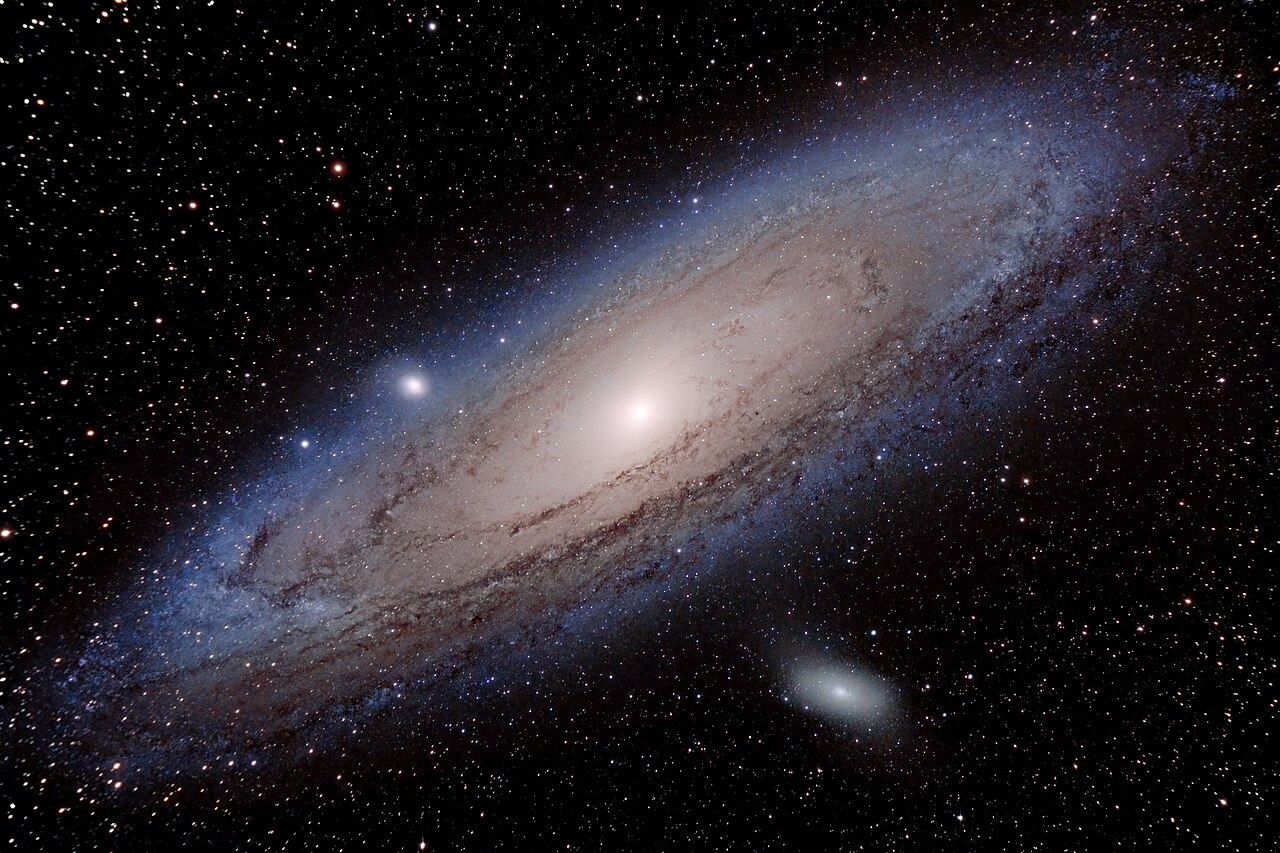
\includegraphics[width=\textwidth]{images/andromeda_main.jpg}

\smallskip
\small Andromeda Galaxy (M31)\\
2.5 million light-years away\\
\tiny Credit: Wikimedia Commons, CC BY-SA 4.0
\end{center}
\end{column}
\end{columns}

\end{frame}

% ============================================================
\begin{frame}{How Big Is Andromeda in the Sky?}

\begin{columns}
\begin{column}{0.55\textwidth}
\begin{center}
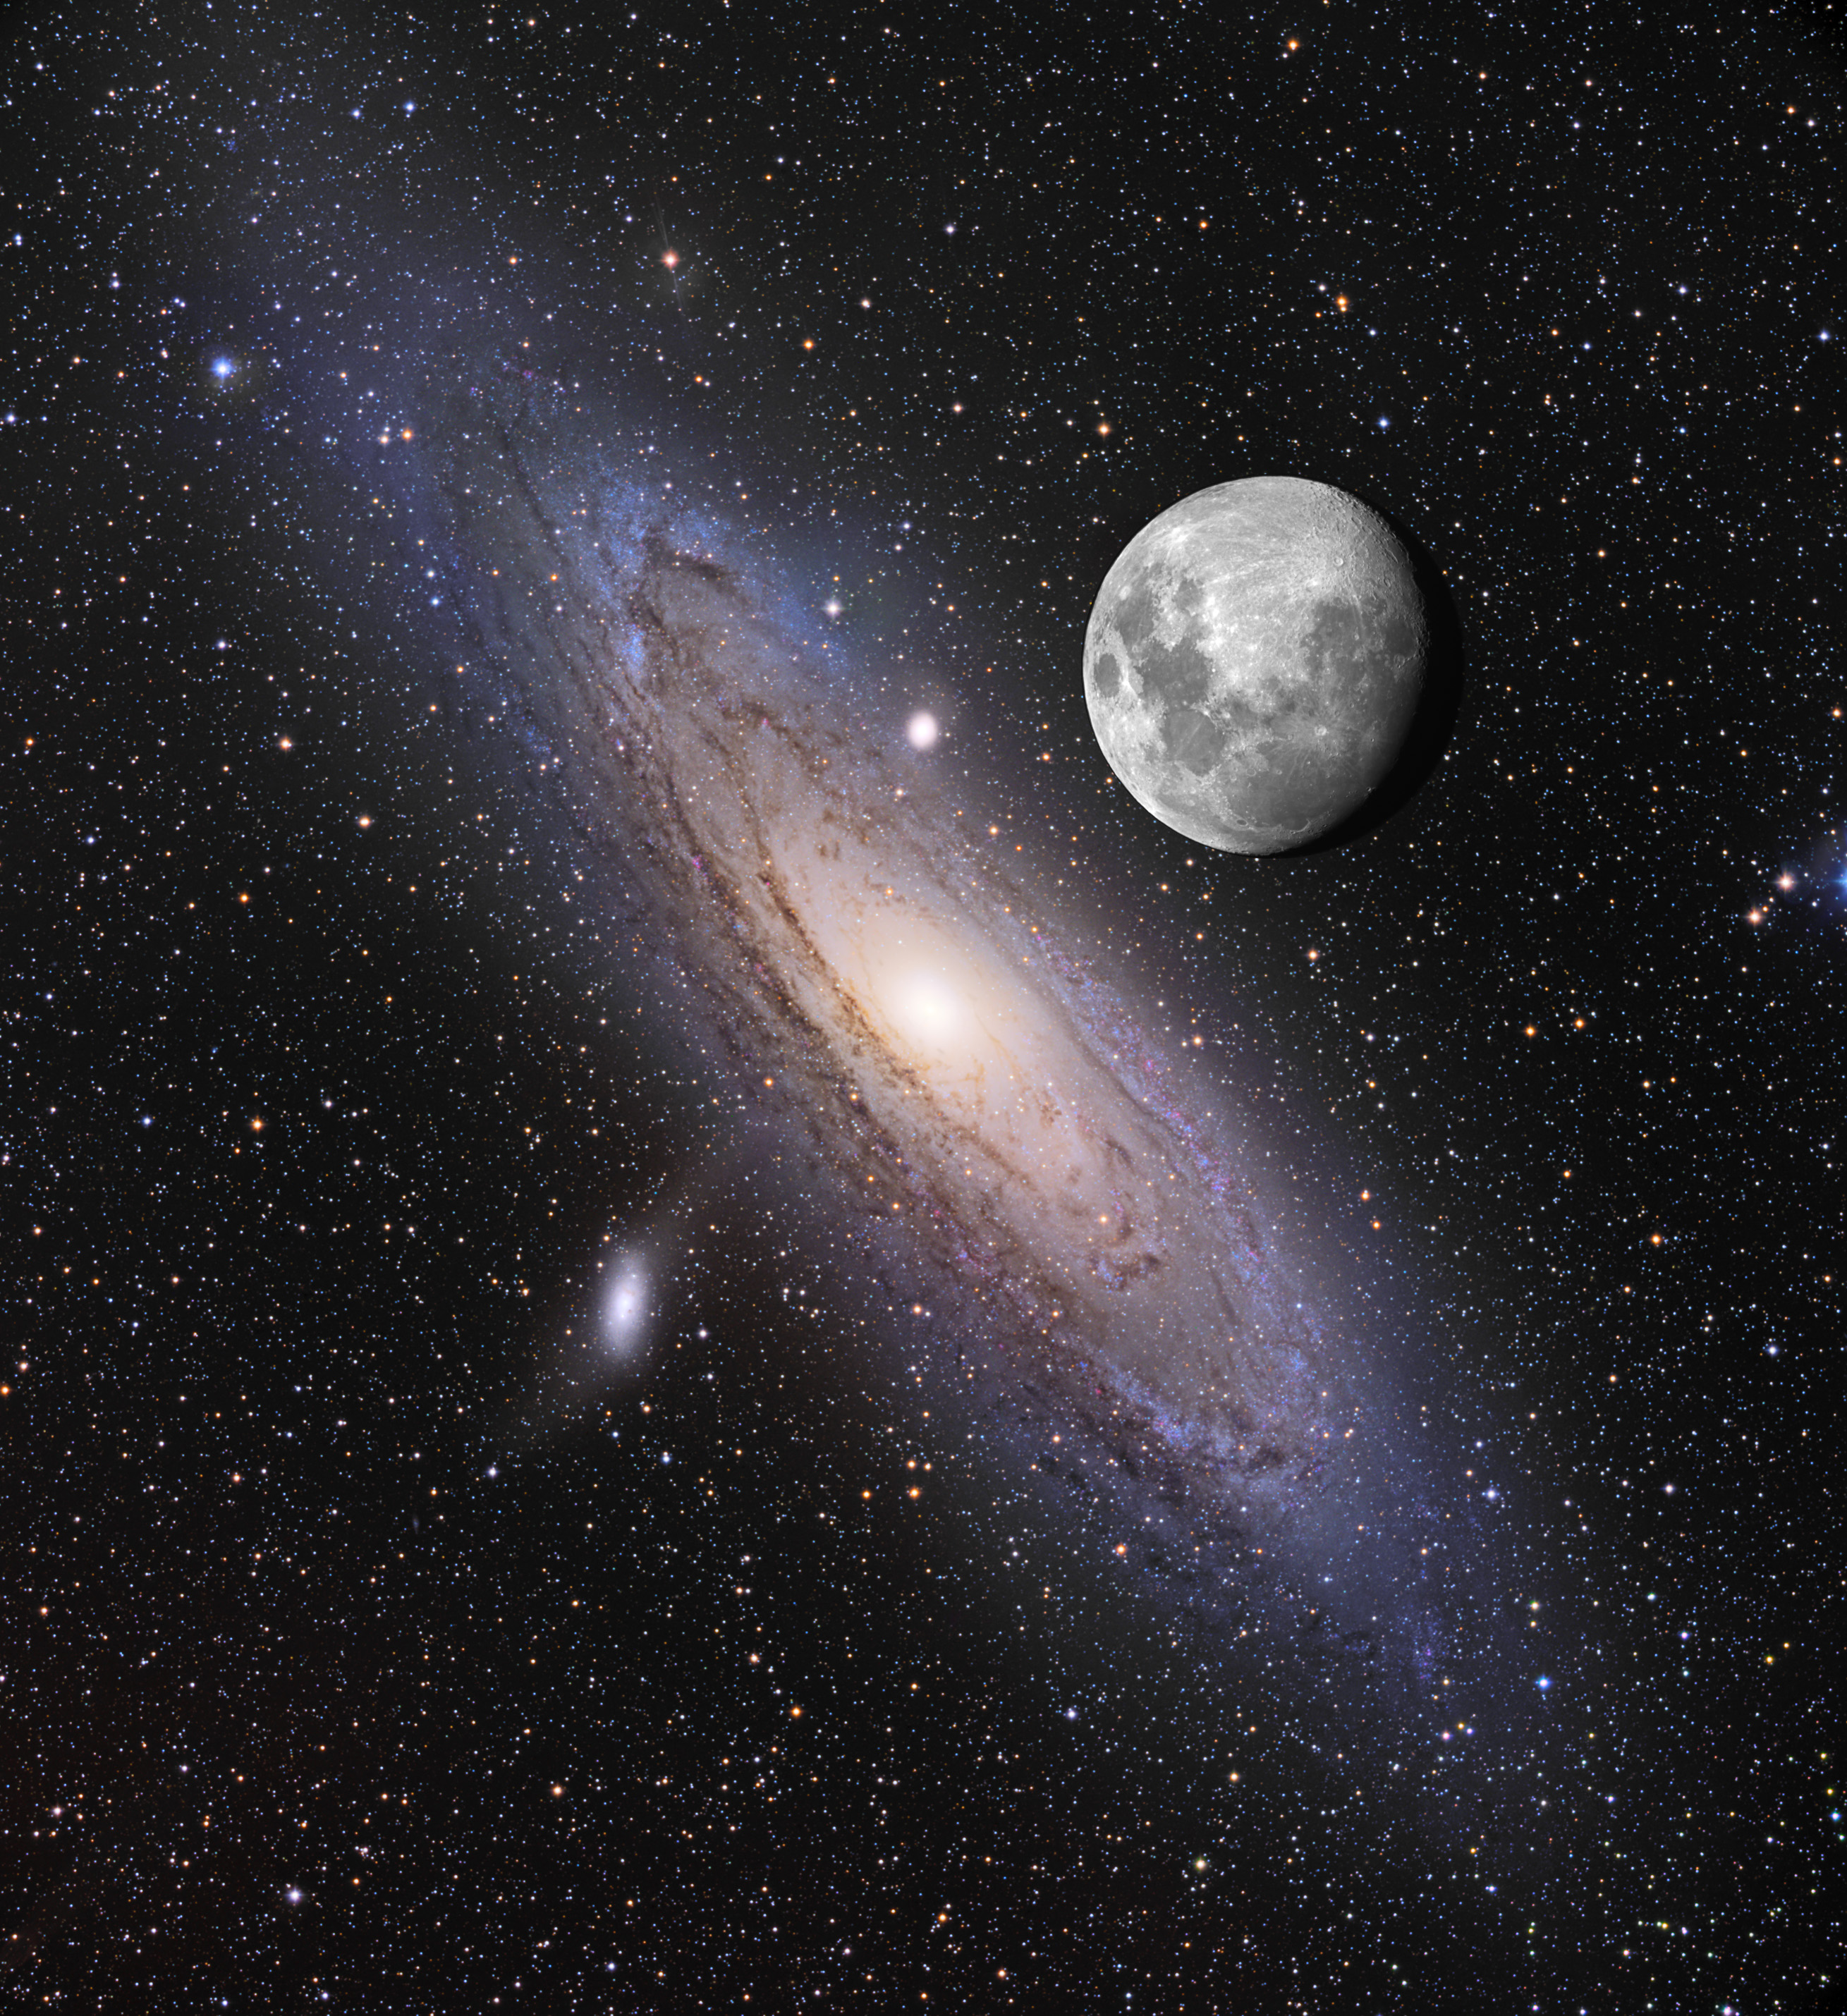
\includegraphics[width=\textwidth]{images/andromeda.jpg}

\smallskip
\tiny Credit: Adam Block, Tim Puckett (APOD)
\end{center}
\end{column}
\begin{column}{0.43\textwidth}
\begin{itemize}
    \item Andromeda and the Moon shown at the \textbf{same scale}
    \item The galaxy is \textbf{several times wider} than the full Moon
    \item But its light is so faint we cannot see it with our eyes
\end{itemize}
\end{column}
\end{columns}

\end{frame}

% ============================================================
\begin{frame}{How Far? --- The Solar System}

\begin{center}
\Large If the Sun were a \textbf{basketball}\ldots
\end{center}

\bigskip

\begin{tabular}{lcc}
\toprule
\textbf{Object} & \textbf{Size} & \textbf{Distance} \\
\midrule
Sun          & Basketball (24\,cm)  & --- \\
Earth        & Peppercorn (2\,mm)   & 26\,m \\
Jupiter      & Walnut (2.4\,cm)     & 134\,m \\
Saturn       & Acorn (2\,cm)        & 247\,m \\
Neptune      & Peanut (8\,mm)       & 774\,m \\
\midrule
Nearest star & Another basketball   & \textbf{6{,}900\,km} \\
\bottomrule
\end{tabular}

\end{frame}

% ============================================================
\begin{frame}{How Far? --- The Galaxy}

\begin{center}
\Large If the Solar System were a \textbf{small coin}\ldots
\end{center}

\bigskip

\begin{itemize}
    \item The \textbf{Milky Way} would be the size of \textbf{Cambridge} ($\sim$20\,km)
    \item The \textbf{Andromeda Galaxy} would be near \textbf{Edinburgh} ($\sim$500\,km)
    \item The coin contains \textbf{our Sun} and all 8 planets
    \item The galaxy contains \textbf{$\sim$100 billion} such coins
\end{itemize}

\end{frame}

% ============================================================
\begin{frame}{The Milky Way --- Our Home Galaxy}

\begin{columns}
\begin{column}{0.55\textwidth}
\begin{itemize}
    \item A spiral galaxy
    \item Diameter: $\sim$100{,}000 light-years
    \item $\sim$100 billion stars
    \item Our Sun is about 26{,}000 light-years from the centre
    \item One orbit around the centre takes $\sim$230 million years
\end{itemize}
\end{column}
\begin{column}{0.45\textwidth}
\begin{center}
\includegraphics[width=\textwidth]{images/milkyway.jpg}

\smallskip
\small UGC\,12158 --- believed to look\\similar to the Milky Way\\
\tiny Credit: ESA/Hubble \& NASA
\end{center}
\end{column}
\end{columns}

\end{frame}

% ============================================================
\begin{frame}{Star Catalogues Through History}

\begin{tabular}{lrc}
\toprule
\textbf{Catalogue} & \textbf{Stars} & \textbf{Year} \\
\midrule
Hipparchus           & $\sim$850        & $\sim$129\,BC \\
Ptolemy (Almagest)   & $\sim$1{,}022    & $\sim$150\,AD \\
Ulugh Beg            & $\sim$994        & 1437 \\
Tycho Brahe          & $\sim$1{,}000    & $\sim$1600 \\
John Flamsteed       & $\sim$2{,}935    & 1725 \\
\midrule
Hipparcos (satellite)& 118{,}218       & 1997 \\
\textbf{Gaia (satellite)} & \textbf{$\sim$2 billion} & \textbf{2022+} \\
\bottomrule
\end{tabular}

\bigskip

\begin{center}
From 850 stars to 2{,}000{,}000{,}000 stars --- in 2{,}000 years
\end{center}

\end{frame}

% ============================================================
\begin{frame}{What Is Gaia?}

\begin{columns}
\begin{column}{0.55\textwidth}
\begin{itemize}\setlength{\itemsep}{2pt}
    \item Space telescope launched by \textbf{ESA} in 2013
    \item Operated \textbf{11 years} (double the planned 5)
    \item Located at \textbf{L2}, 1.5 million\,km from Earth
    \item Last observation: Jan 2025
    \item Measured for each star:
    \begin{itemize}\setlength{\itemsep}{1pt}
        \item \textbf{Position} and \textbf{distance}
        \item \textbf{Motion} (speed and direction)
        \item \textbf{Colour} and \textbf{brightness}
    \end{itemize}
\end{itemize}
\end{column}
\begin{column}{0.43\textwidth}
\begin{center}
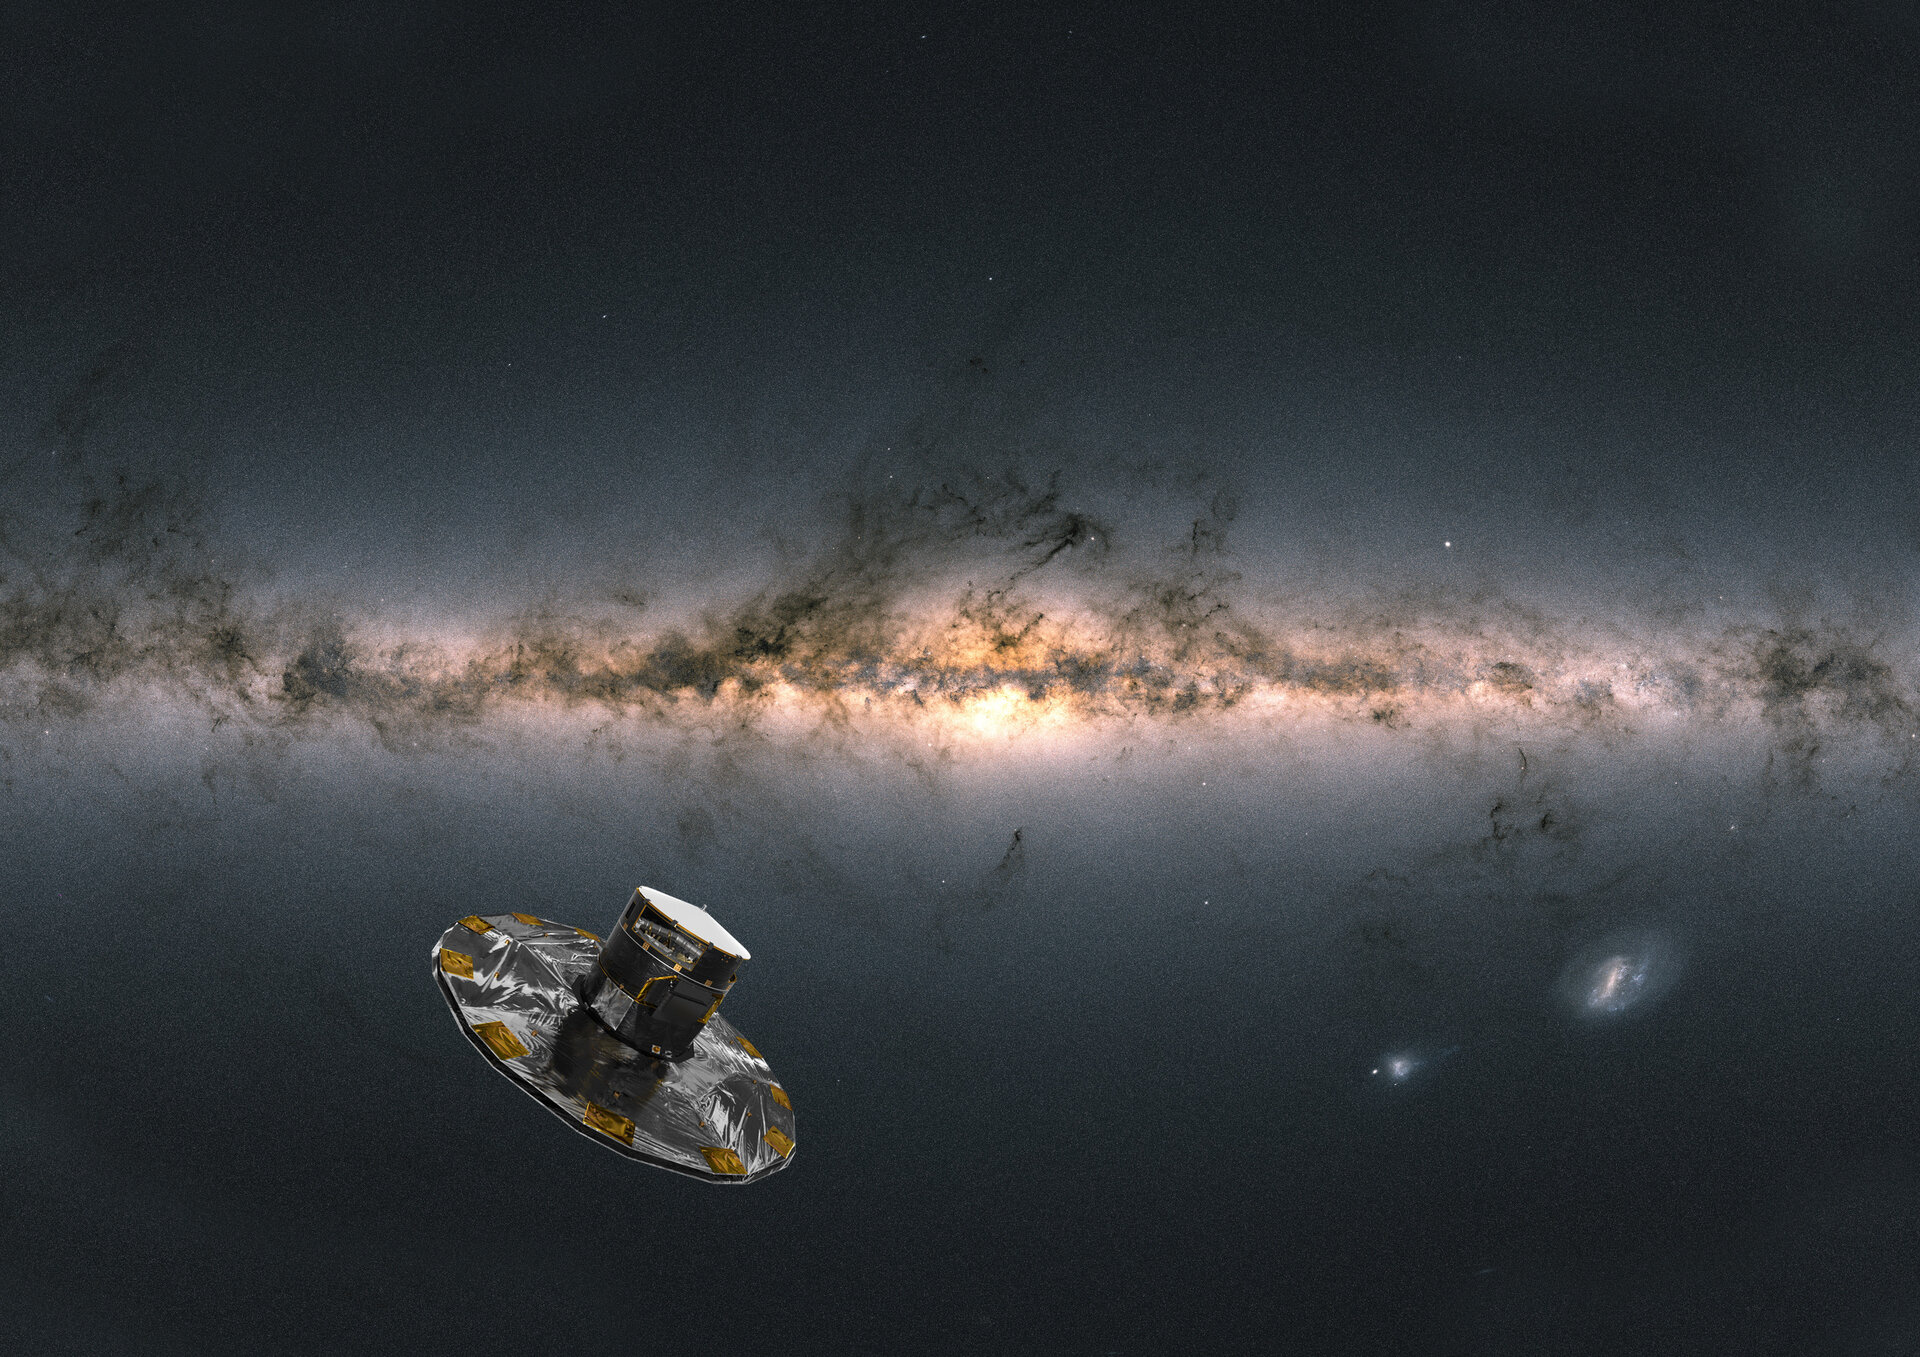
\includegraphics[width=\textwidth]{images/gaia_satellite.jpg}

\smallskip
\tiny Credit: ESA, via gaia.ac.uk
\end{center}
\end{column}
\end{columns}

\end{frame}

% ============================================================
\begin{frame}{Lagrange Point L2}

\begin{columns}
\begin{column}{0.55\textwidth}
\begin{center}
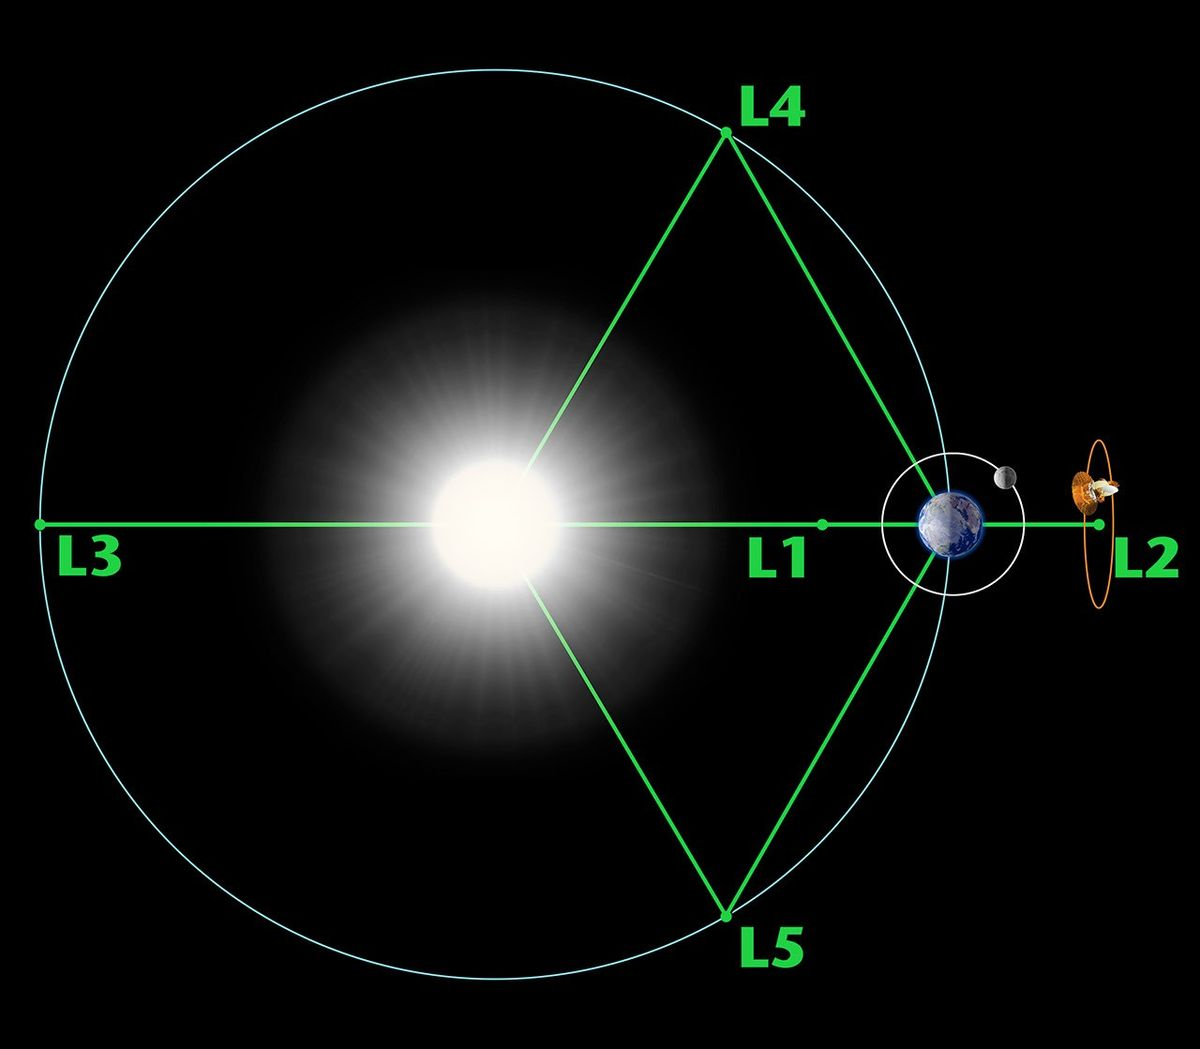
\includegraphics[width=\textwidth]{images/lagrange.jpg}

\smallskip
\tiny Credit: NASA/WMAP Science Team
\end{center}
\end{column}
\begin{column}{0.43\textwidth}
\begin{itemize}
    \item At L2, gravity of Sun and Earth together kept Gaia in a stable orbit
    \item Always on the \textbf{night side} of Earth --- good for observing stars
    \item Sun, Earth, and Moon were all behind Gaia's sunshield
\end{itemize}
\end{column}
\end{columns}

\end{frame}

% ============================================================
\begin{frame}{How Gaia Scans the Sky}

\begin{itemize}
    \item Two telescopes separated by \textbf{106.5\textdegree}
    \item Gaia \textbf{spun} once every 6 hours
    \item The spin axis slowly \textbf{precessed} every $\sim$63 days
    \item This scanning pattern covered the \textbf{entire sky}
    \item Each star observed about \textbf{70+ times} over 11 years
    \item Camera: \textbf{1 billion pixels} (106 CCDs) --- largest ever in space
\end{itemize}

\end{frame}

% ============================================================
\begin{frame}{Gaia's Results}

\begin{columns}
\begin{column}{0.48\textwidth}
\begin{itemize}
    \item \textbf{Data Release 3} (June 2022):
    \begin{itemize}
        \item $\sim$\textbf{1.8 billion} stars
        \item Distances for $\sim$1.5 billion
        \item Motions for $\sim$1.5 billion
        \item Also: asteroids, galaxies, quasars
    \end{itemize}
    \smallskip
    \item \textbf{DR4} expected late 2026
    \item \textbf{DR5} (final) $\sim$2030
    \smallskip
    \item Over \textbf{12{,}000 papers} published
\end{itemize}
\end{column}
\begin{column}{0.50\textwidth}
\begin{center}
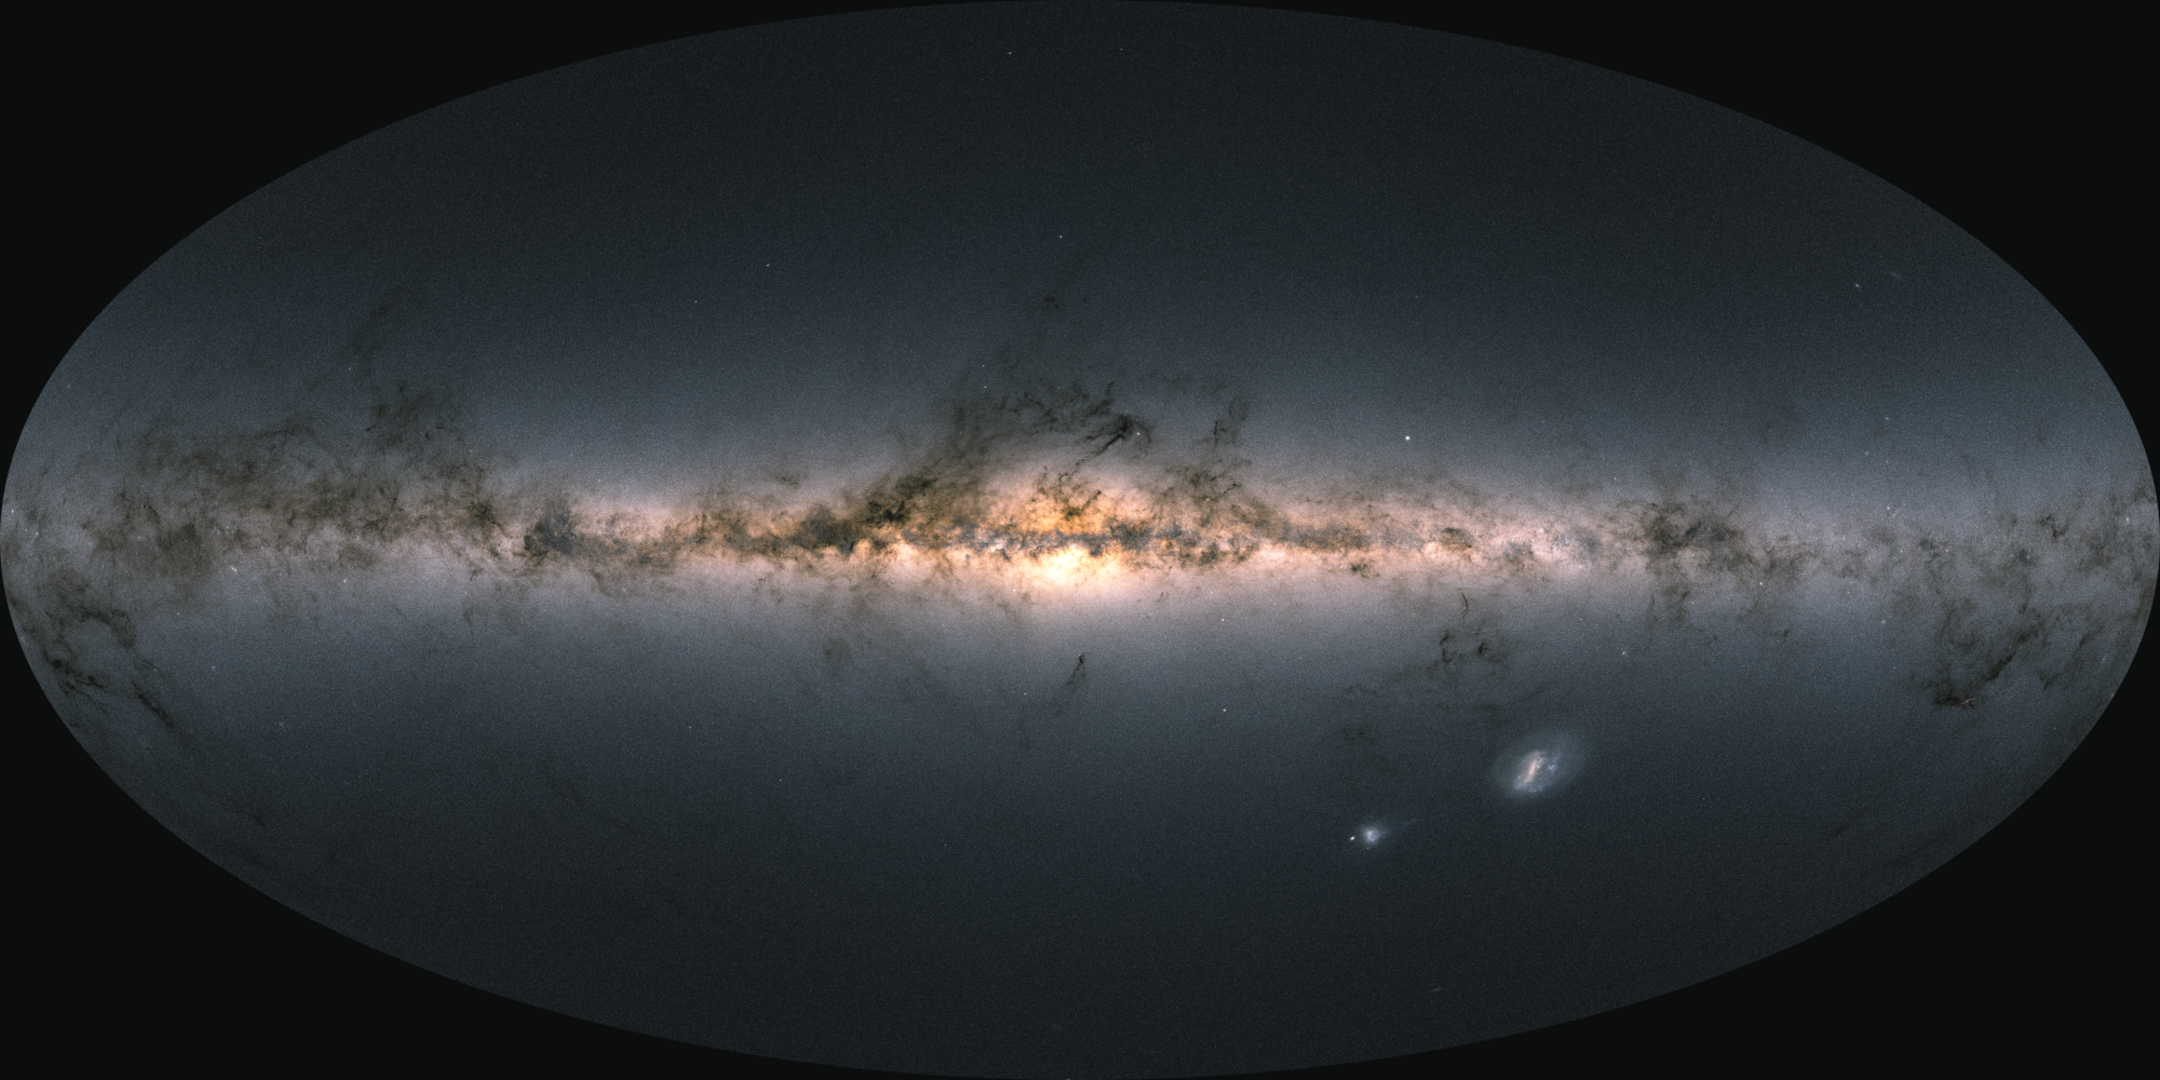
\includegraphics[width=\textwidth]{images/gaia_skymap.png}

\smallskip
\small Each dot is a star measured by Gaia.\\
Colour = real star colour (blue = hot, red = cool).\\
The bright band is the Milky Way's disc seen from inside.\\
\tiny Credit: ESA/Gaia/DPAC
\end{center}
\end{column}
\end{columns}

\end{frame}

% ============================================================
\begin{frame}{The Legacy of Star Catalogues}

\begin{center}
\Large
Hipparchus's catalogue from 129\,BC\\
was still used \textbf{1{,}500 years later}
\end{center}

\bigskip

\begin{itemize}
    \item Tycho Brahe's data led Kepler to discover the \textbf{laws of planetary motion}
    \item The Hipparcos catalogue is still used today, \textbf{30 years} after publication
    \item Gaia's catalogue will serve astronomy for \textbf{decades to come}
\end{itemize}

\bigskip

\begin{center}
\large\itshape
There is a special satisfaction in knowing\\
your work will be used long after you finish it.
\end{center}

\end{frame}

% ============================================================
\begin{frame}{}

\begin{center}
\Huge Thank you!

\bigskip
\Large Questions?

\bigskip
\bigskip
\normalsize
Michael Nedzelsky\\
Institute of Astronomy, Cambridge\\
\texttt{gaia.ac.uk}
\end{center}

\end{frame}

\end{document}
